%%%
%%%    Copyright (c)  2002  Peter Biechele, Francesco Petruccione
%%%
%%%    Permission is granted to copy, distribute and/or modify this document
%%%    under the terms of the GNU Free Documentation License, Version 1.1
%%%    or any later version published by the Free Software Foundation;
%%%    with no Invariant Sections, with the Front-Cover Texts being 
%%%    FRONT LIST, and with the Back-Cover Texts being BACK LIST.
%%%    A copy of the license is included in the section entitled "GNU
%%%    Free Documentation License".
%%%
%
% Short Summary of all Java Features
%

\chapter{Summary of Java}

\section{Basic Syntax}
\begin{center}
  \begin{tabular}{l>{\small}l}
    Documentation & \verb|/** Javadoc documentation */| \\
    Comments & \verb|/* Multi Line Comments */| \\
             & \verb|// Single Line Comments| \\
    Constants & \verb|final int i = 10; | \\
    Logical Operators & \verb% !, &, |, ^, &&, || % \\
    Integer data types & \verb|byte, short, int, long| \\
    Floating point data types & \verb|float, double| \\
    Arithmetic Operators & \verb|+, -, *, /, %, ++, --|\\
    Bitwise Operators & \verb%~, &, |, ^, <<, >>, >>> % \\
    Comparison Operators & \verb|<, <=, >, >=, ==, != | \\
    Flow Control & \verb|if () ... else ... | \\
                 & \verb|... ? ...  :   ... | \\
                 & \verb|switch() { case .. : ...; break; default: ... } | \\
                 & \verb|for (.. ; .. ; ..) { ...; } | \\
                 & \verb|while () { ...;} | \\
                 & \verb|do { ...; } while (); | \\
  \end{tabular}
\end{center}

\section{Structure of a Java program}
The general structure of a Java program is:
\begin{itemize}
\item package
\item import
\item Classes
\item Interfaces
\end{itemize}
\begin{figure}[h]
  \begin{center}
 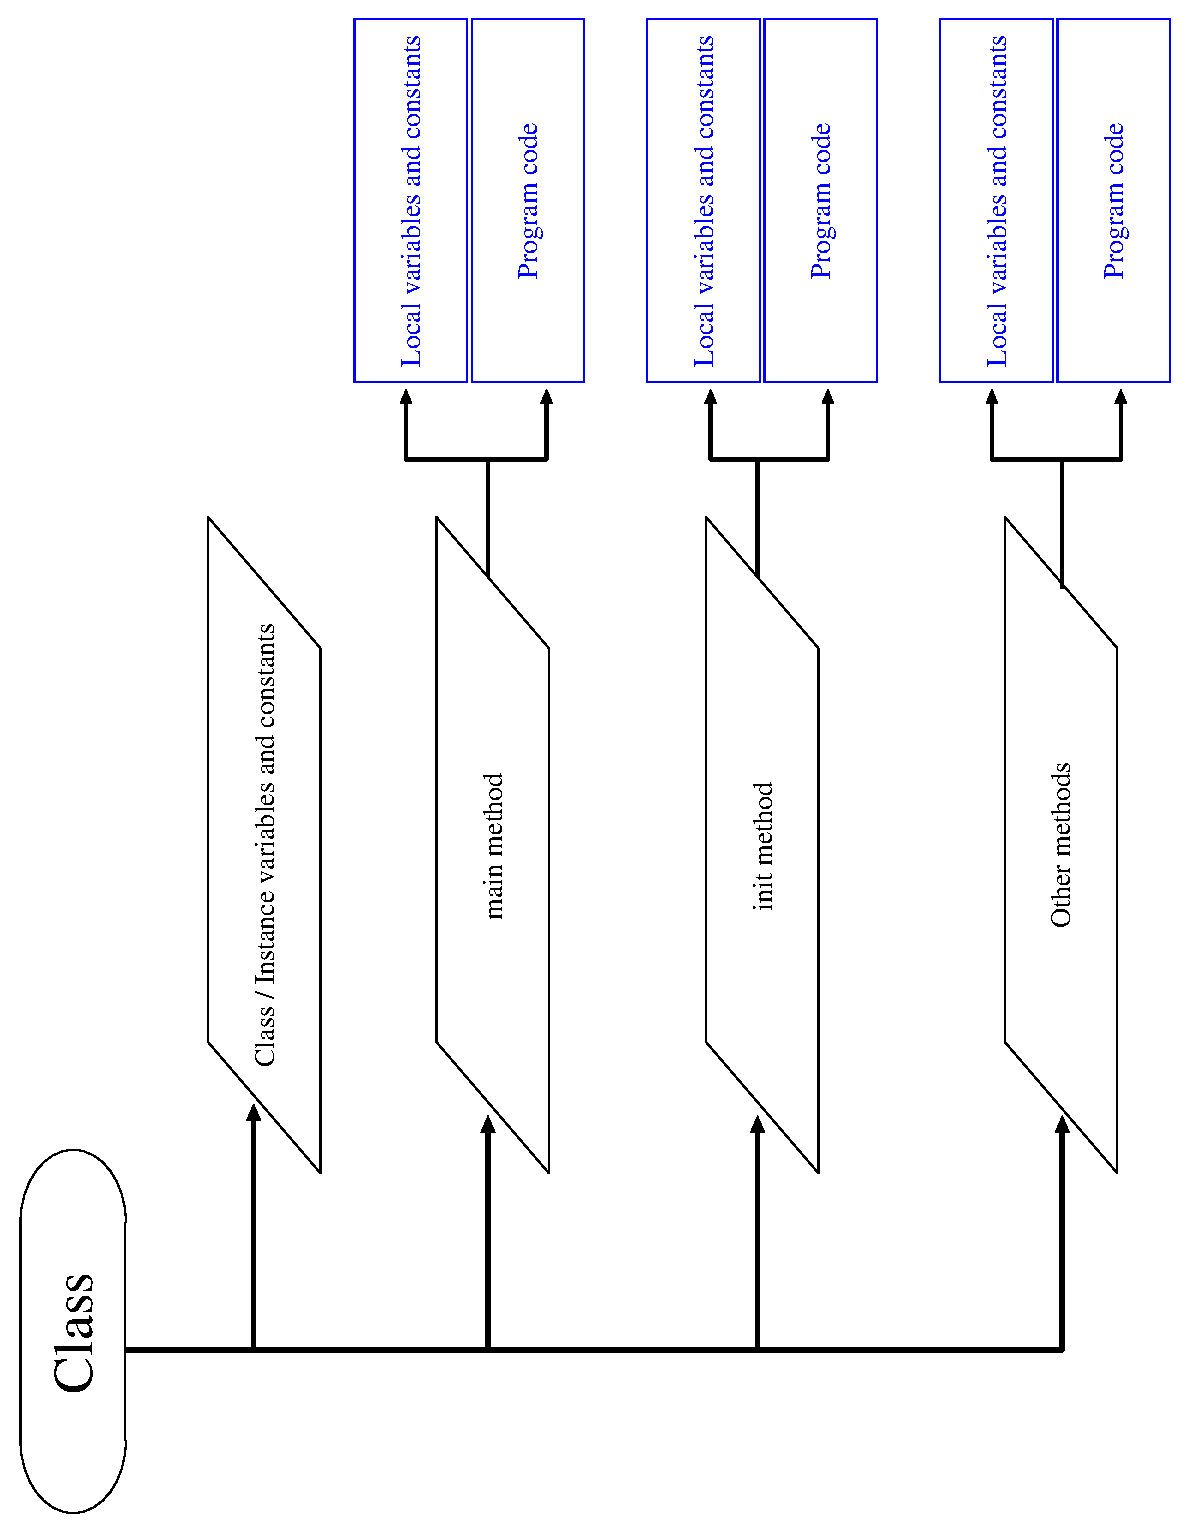
\includegraphics[angle=-90,width=.8\textwidth]{ClassStructure.eps}
 \caption{The class structure of a Java program, either application or an applet.}
 \label{fig:ClassStructure}
  \end{center}
\end{figure}

\section{The \texttt{java.lang.System} class}
%%\begin{table}[htbp]
  \begin{center}
    \begin{tabular}{lp{5cm}p{.5\textwidth}}
      Type & Field & Description \\\hline
      PrintStream & err & standard error output stream \\
      InputStream & in & standard input stream \\
      PrintStream & out & standard output stream \\ \hline\hline
      modifier & method & explanation \\\hline
      static void & \verb|arraycopy(Object src, int srcpos, Object dst,| 
                    \verb|int dstpos, int length)| &
         Copies an array from the specified source array, beginning at 
         the specified position, to the specified position of the
         destination array. \\
      static void & \verb|exit(int status)| & Terminates the currently 
                                     running Java Virtual Machine.\\
      static void & \verb|setErr(PrintStream err)| &  
                   Reassigns the "standard" error output stream.\\
      static void & \verb|setIn(InputStream err)| &  
                   Reassigns the "standard" input output stream.\\
      static void & \verb|setOut(PrintStream err)| &  
                   Reassigns the "standard" output output stream.\\
      static String & \verb|getProperty(String key)| & get the system property
                            defined by the given key. \\
      static String & \verb|setProperty(String key)| & set the system property
                            defined by the given key. \\
    \end{tabular}
%%    \caption{Important fields and methods of the System class.}
%%    \label{tab:SystemClass}
  \end{center}
%%\end{table}

\section{Mathematics}
\subsection{The \texttt{java.lang.Math} class}
\subsection{JNL}
\subsection{JavaSci}
\subsection{Others}
\label{sec:Others}
\section{Random Numbers}
\section{Keyboard input and Screen Output}
\section{File I/O}
\section{Ptplot}
\section{AWT}
\section{Conversions and Casting}
\section{Threads}
\section{Printing}
\section{Modifiers}
%%\begin{table}[htbp]
  \begin{center}
    \begin{tabular}{ll}
      abstract method & A method having no body of code. The code can
        be implemented in a subclass.\\
      abstract class & A class containing at least one abstract method \\
      interface & A class, where all defined methods are abstract by default.
        No variables only constants are possible in interfaces. Interfaces
        have to be implemented, not subclassed, and all methods have to be
        overridden otherwise it must be declared abstract.\\
    \end{tabular}
%%    \label{tab:Modifiers}
  \end{center}
%%\end{table}
\section{Debugger}
\section{JDE and Emacs}

%%% Local Variables: 
%%% mode: latex
%%% TeX-master: "V_98"
%%% End: 
